\documentclass{article}

\usepackage[usenames]{color} 
\usepackage{graphicx} 


\newcommand{\todo}[1]{\textcolor{red}{\textbf{TODO: }\it{#1}}}
\newcommand{\inhoud}[1]{\textcolor{blue}{\textbf{Summary: }\it{#1}}}
\newcommand{\revise}[1]{\textcolor{orange}{\textbf{Revise: }\it{#1}}}

\definecolor{MyDarkGreen}{rgb}{0.13, 0.54,0.13} 
\newcommand{\voegtoe}[1]{\textcolor{MyDarkGreen}{\textbf{-Insert: }\it{#1}}\newline}

\title{Real-time spatial growth model map generation}
\author{Ruud op den Kelder}

\begin{document}

\maketitle

\begin{abstract}
The abstract of Real-time spatial growth model based map generation
\end{abstract}
\newpage 

\tableofcontents
\newpage 

\section{Introduction}
\inhoud{Introduction zo snel mogelijk maken. saai werk en beschrijven van context /previous work 
geeft goeie basis om verder op te werken. }

\todo{snel maken, dan ben je er voorlopig vanaf}

This thesis discusses and utilizes techniques from geometric and biological modelling for the procedural generation of 2D enviroments, with an emphasize on game environments. The techniques used in this paper are greatly influenced by the field of procedural city generation and the more mature field of procedural generation of plants and trees. 

The research which preceded this document strived to construct a intuitive organic modelling method for the creation of 2D maps. The central focus of this research has been on adapting, constructing and implementing real-time \emph{communicating} growth models using two types of dynamic structures. These two types can be described as network type structures, using l-systems and map l-systems, and 2D 2 manifold shaped structures, using techniques derived from cellular automata and cell systems.     

\subsection{Procedural Modeling}
\inhoud{beschrijf kort geschiedenis van procedural modeling en werk naar map generation}
\cite{citysurvey}



\subsection{L-systems}
\inhoud{beschrijf toepassingen van L-systems}

\subsection{Map generation}
\inhoud{beschrijf huidige games en tools die gebruik maken van procedural generation voor geometrie van virtuele werelden.}

\subsubsection{spatial growth based}
\inhoud{verhaal over het feit dat spatial growth based-user controlled bouwen van maps relatief nieuw is.}

\subsubsection{Interactivity}
\inhoud{beschrijf tools voor het manipuleren van modellen die afhankelijk zijn van l-systems en tools die worden 
	gebruikt voor level design, zoals tools voor terrain editors.}


\subsection{Adding simple gameplay properties}

\subsection{The growth model map generator tool}

%inspiratie:
%\begin{figure}
%  \begin{center}
%    \subfigure[global map impression]{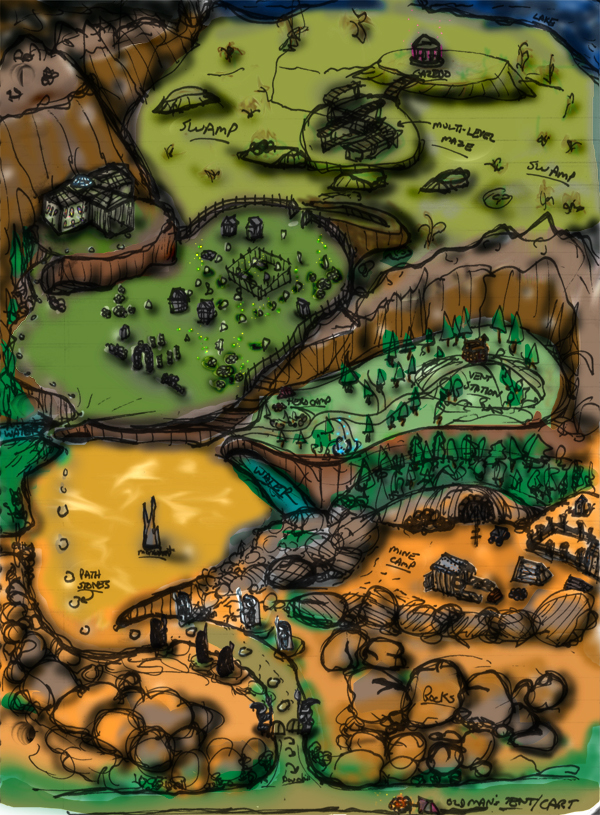
\includegraphics{images/map_design.jpg}}
%    \subfigure[abstract city,road network %impression]{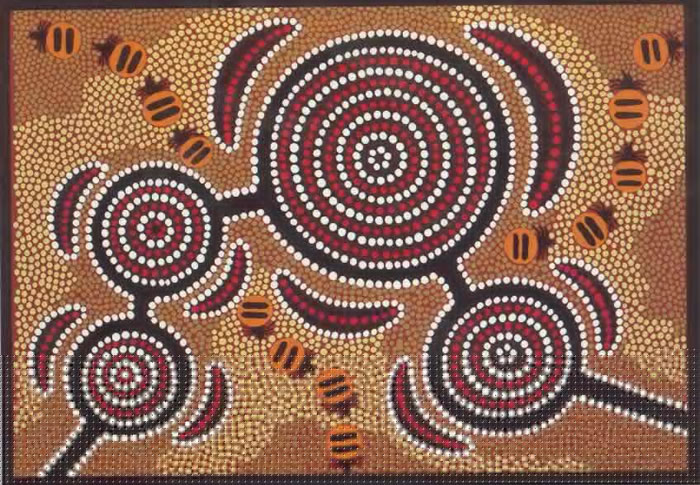
\includegraphics{images/aboriginal_art.jpg}}
%	\subfigure[afforestation representation impression]{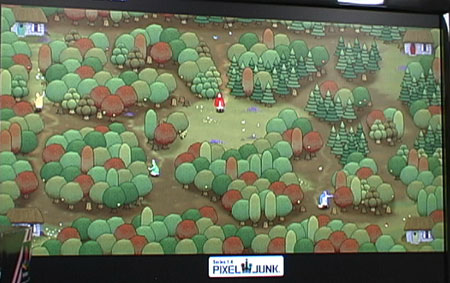
\includegraphics{images/forest.jpg}}
%  \end{center}
%  \caption{Collage of impressions}\label{fig:impressions}
%\end{figure}

tijdelijk: 

\begin{figure}
\centering
  \begin{center}
	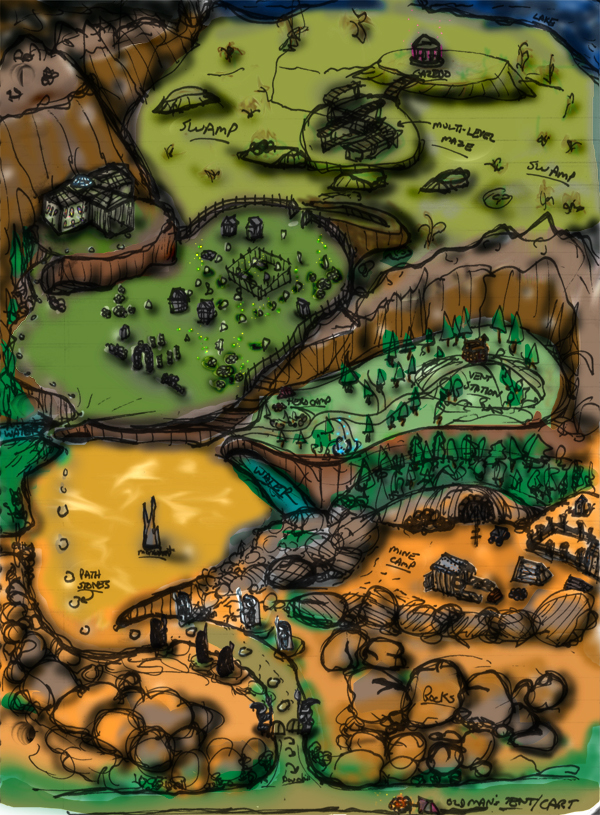
\includegraphics[width=200pt]{images/map_design.jpg}
	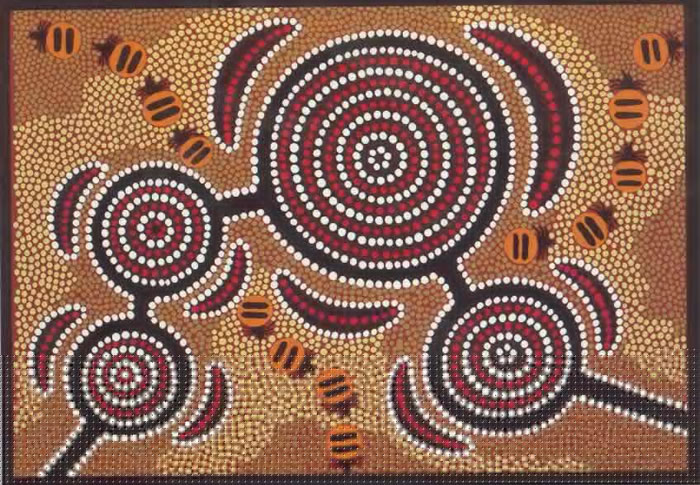
\includegraphics[width=200pt]{images/aboriginal_art.jpg}
	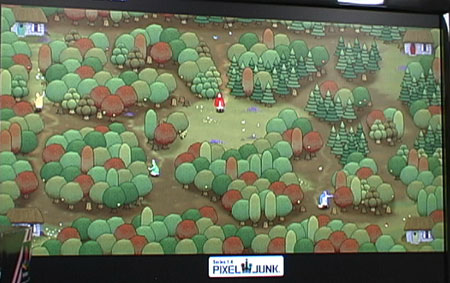
\includegraphics[width=200pt]{images/forest.jpg}
\end{center}
	\caption{impressions}\label{fig:global_map}
\end{figure}


\section{Method: realtime spatial growth models}

\subsection{dynamical systems: polygonal surfaces}
\inhoud{2D polygonale expansie van een ondergrond model als land of water die wordt gestuurd door eigenschappen van het type maar ook door ruimtelijke manipulatie methodes zoals vectorfields. representatie(onder voorbehoud): 
\begin{itemize}
\item Cellular automata
\item Cell systems
\item iets wat niet met cellen werkt  
\end{itemize}
realtime hertriangulatie zal moeten worden toegepast. 
polygonal meshes: 
\begin{itemize}
\item representation for irregular 2D volumes.  
\item suitable for water, land, cave like structures  
\item real-time demand, so need for efficient algorithms
\item houdt rekening met triangulatie
\item houdt rekening met smoothing
\item datastructure
\end{itemize}
citeer: On Vertex-Vertex Systems and Their Use in
Geometric and Biological Modelling
}

\todo{dit kan al snel worden geimplementeerd dus logisch om dit als eerste te beschrijven en methode uit te werken.}

\voegtoe{beschrijf waarom ik dynamic modeling technieken nodig heb}



\voegtoe{review methodes for dynamic modeling}


\voegtoe{focus op cell systems}


\voegtoe{custom systeem dat alle eigenschappen heeft die nodig zijn voor de polygonale expansie}



\cite{compgeom}
\cite{vertexsystems}

\begin{figure}
\centering
  \begin{center}
	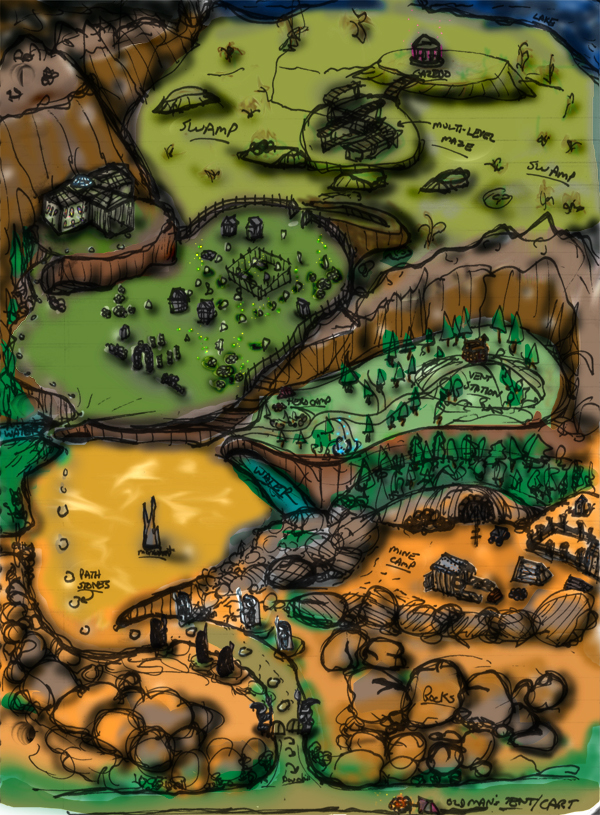
\includegraphics[width=200pt]{images/map_design.jpg}
	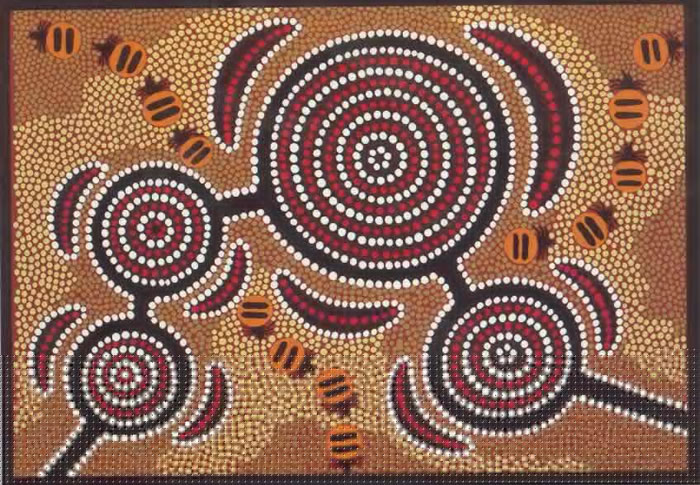
\includegraphics[width=200pt]{images/aboriginal_art.jpg}
	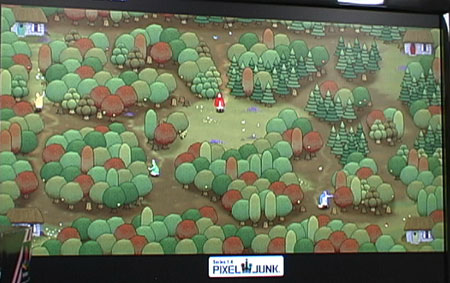
\includegraphics[width=200pt]{images/forest.jpg}
\end{center}
	\caption{impressions}\label{fig:global_map}
\end{figure}




\subsection{l-systems and map l-system type spatial growth patterns}

\cite{lcreport}


\subsection{Real-Time spatial growth Models For Outdoor Areas}
\inhoud{Per type spatial growth model bespreken wat de context is binnen outdoor areas en dus met 
welke andere spatial growth modellen het communiceert en welke effecten het spatial growth model heeft 
op de andere en vica versa. Ook bespreken op wat voor manier een vector field (en andere tools 
die invloed hebben op de ruimtelijke indeling)  effect heeft op de uitdijing van dit type model.   
}

\subsubsection{Land} 
\todo{beschrijven hoe land expansie verloopt en hoe het communiceert met andere modellen}


\subsubsection{Water} 

\subsubsection{Roads}

\subsubsection{Afforestation} 

\subsection{Real-time spatial growth models For Indoor Areas}

\subsubsection{Caves}

\subsubsection{Canarian Aboriginal style homes}

\section{Organic map generation tool}

\subsection{Modifiers}

\subsubsection{Spatial modifiers}

\inhoud{
\begin{itemize}
\item vector fields: dit moet je wellicht helemaal aan het begin doen omdat alle spatial growth models
gemanipuleerd worden door deze vector fields.
\item obstruction with solid objects
\item smudge-like tool
\end{itemize}
}

\subsubsection{Timeflow modifiers}
\inhoud{
\begin{itemize}
\item pause model
\item speed up model
\item slow down model
\item reverse time flow
\end{itemize}
}


\subsection{User controlled map generation}

\subsection{automatic map generation} 


\section{Implementation}
\subsection{Tools used}
\inhoud{ 
\begin{itemize}
\item programming language: c++ (for now)
\item visualization library: openGL or Ogre3D (if it features easy vertex manipulation) 
\item physics engine: ODE (onder voorbehoud)  
\item collision detection: D-Collide (onder voorbehoud)
\end{itemize}
}

\subsection{Application Class Structure}
\subsection{User Interface}
\subsection{Communication system between models}

\section{Results}

\section{Conclusion}





%references
%logische volgorde:
%introduction: context-> previous work  
%method
%implementation
%results 
%conclusion 
\newpage 
\bibliographystyle{abbrv}	% (uses file "plain.bst")
\bibliography{thesisrefs}	% expects file "myrefs.bib"

\end{document}

